\documentclass[a4paper,11pt,noarxiv]{quantumarticle}
\usepackage[utf8]{inputenc}
\usepackage[english]{babel}
\usepackage[T1]{fontenc}
\usepackage{amsmath,amssymb,amsthm}
\usepackage{graphicx}
\usepackage{booktabs}
\usepackage{hyperref}
\usepackage{tikz}

\newtheorem{theorem}{Theorem}
\newtheorem{lemma}{Lemma}
\newtheorem{observation}{Observation}

\newcommand{\tc}{\mathrm{tc}}
\newcommand{\sczz}{\mathrm{sc}}
\newcommand{\bnd}[1]{\partial #1}

% DRAFT v0.1 (2026-07-23). Body drafted per telegram outline; abstract and
% introduction are rough per workflow phase 3; polish passes pending.

\begin{document}

\title{How close to optimal are tensor-network contraction orders? Certified bounds and a reproducible frontier at fixed budgets}

\author{Jin-Guo Liu}
\affiliation{Advanced Materials Thrust and Quantum Science and Technology Center,
The Hong Kong University of Science and Technology (Guangzhou), Guangzhou, China}

\begin{abstract}
Contraction-order optimizers determine the cost of tensor-network computation,
yet they are benchmarked only against each other, so it is unknown how far
their output lies from the true optimum. We establish a reproducible
fixed-budget frontier on two representative instances---a random 3-regular
network and a Sycamore-style random-circuit proxy---and certify how close to
optimal it is. Ten mechanistically distinct search algorithms and two
independent toolchains (\textsf{omeco}/TreeSA and \textsf{cotengra}) converge
to a common contraction-cost frontier at matched 90-second budgets, which is
unchanged by a tenfold budget increase. Combining a rigorous sum-form
isoperimetric bound, treewidth minor certificates, and a balanced-cut argument
with an explicit temporal cut, we localize the Sycamore-proxy optimum to
$[53, 61.544]$ in $\log_2$ floating-point operations and prove the frontier is
width-optimal. We further prove that \emph{no} bound depending only on the
isoperimetric profile can exceed the bisection width, so the remaining gap of
$8.5\approx\log_2 n$ bits---the multiplicity of near-maximal contractions---is
invisible to all width-type arguments; measurements show this multiplicity
behaves as a conserved quantity under profile reshaping. Finally, we exhibit a
cautionary failure mode: eight novel algorithms appeared to outperform the
baseline by up to $800\times$ until a single mis-tuned baseline parameter
(\texttt{sc\_target}) was fixed, after which the tuned baseline explained the
entire gain; the fix now ships in the \textsf{omeco} library. Certification,
not further mechanism search, is the missing axis of contraction-order
benchmarking.
\end{abstract}

\maketitle

\section{Introduction}
\label{sec:intro}

The cost of simulating a quantum circuit---or of any tensor-network (TN)
computation---is set not by the network alone but by the order in which it is
contracted. A good contraction tree can be exponentially cheaper than a poor
one, and a rich ecosystem of optimizers has grown around this fact: greedy and
cost-portfolio heuristics~\cite{orgler_2024_optimizing,pfeifer_2013_faster},
hypergraph partitioning and hyper-optimization~\cite{gray_2020_hyper},
simulated-annealing tree search~\cite{kalachev_2021_multi,anon_2025_optimizing},
treewidth machinery~\cite{markov_2005_simulating,dumitrescu_2018_benchmarking},
and exact-glue hybrids~\cite{ibrahim_2022_constructing,staudt_2024_improved}.
These tools decide the feasibility of state-of-the-art circuit
simulations~\cite{liu_2022_verifying}.

All of them, however, are evaluated the same way: against each other. An
optimizer is ``good'' if it beats another optimizer on a benchmark set. How far
either sits from the \emph{true optimum} of a given instance is, outside of
exactly solvable small cases~\cite{pfeifer_2013_faster}, unknown. The
treewidth literature provides asymptotic and width-type lower
bounds~\cite{markov_2005_simulating}, but these bound the largest single
contraction, not the total floating-point count that practitioners minimize,
and they are rarely computed for concrete benchmark instances.

This paper supplies the missing axis for two representative instances: a
250-tensor random 3-regular network (an expander, the hard regime for
partitioners) and a 561-tensor Sycamore-m20-scale random-circuit proxy. Our
contributions are threefold. First, a \emph{reproducible frontier}: under a
fixed 90-second single-threaded budget with validator-recomputed costs, ten
mechanistically distinct search algorithms and two independent toolchains
converge onto a common contraction cost, which a tenfold budget increase does
not move (Fig.~\ref{fig:convergence}). Second, a \emph{certified bracket}: a
rigorous sum-form isoperimetric bound (Theorem~\ref{thm:sumform}), treewidth
minor certificates, and a balanced-cut argument localize the Sycamore-proxy
optimum to $[53, 61.544]$ bits and prove the frontier width-optimal
(Fig.~\ref{fig:ladder}). Third, an \emph{impossibility observation}: no
function of the isoperimetric profile alone can certify more than the
bisection width (Theorem~\ref{thm:dyadic} and its refutation-by-collapse), so
the residual $\approx\log_2 n$ bits is structural---it counts near-maximal
contractions, a quantity we measure to behave as conserved
(Fig.~\ref{fig:conservation}). Along the way we document a failure mode with
practical consequences: a mis-tuned default in the baseline
(\texttt{sc\_target}) masqueraded as an $800\times$ algorithmic improvement
across eight independently implemented ``novel'' optimizers
(Fig.~\ref{fig:masquerade}), and the corresponding one-line fix now ships in
the \textsf{omeco} library~\cite{omeco}.

\section{Setup}
\label{sec:setup}

\paragraph{Networks as graphs.} Both instances are closed tensor networks with
all bond dimensions~2 and every index shared by exactly two tensors, hence
ordinary graphs $G=(V,E)$ with $n=|V|$ tensors and $m=|E|$ indices. For a
subset $S\subseteq V$, write $\bnd{S}$ for its edge boundary. Because bonds
have dimension 2, the intermediate tensor obtained by contracting the tensors
in $S$ carries exactly the indices $\bnd{S}$, i.e., $|\bnd{S}|$ bits.

\paragraph{Contraction trees and costs.} A contraction order is a binary tree
$T$ whose leaves are the tensors; an internal node $v$ with children carrying
disjoint leaf-sets $A_v, B_v$ produces the intermediate for
$S_v = A_v\cup B_v$. Its contraction ranges over all indices of both children,
costing $2^{\mathrm{cost}_v}$ multiply--adds. We use throughout the log-scale
time and space complexities
\begin{equation}
\tc(T) = \log_2 \sum_v 2^{\mathrm{cost}_v},
\qquad
\sczz(T) = \max_v |\bnd{S_v}|.
\end{equation}

\begin{lemma}[cost identity]
\label{lem:identity}
For every internal node $v$ of a contraction tree over a closed network,
\begin{equation}
\mathrm{cost}_v \;=\; |\bnd{S_v}| + |E(A_v,B_v)| \;\ge\; |\bnd{S_v}|,
\end{equation}
where $E(A,B)$ is the set of edges between $A$ and $B$.
\end{lemma}

\begin{proof}
Classify each edge of $G$ by its endpoints relative to the partition
$S_v = A_v \uplus B_v$: an edge inside $S_v$ has one endpoint in each part
(if both endpoints were in $A_v$ it would not touch the contraction at $v$'s
parent scale; formally it lies in $E(A_v,B_v)$ and in $\bnd{A_v}\cap\bnd{B_v}$);
an edge leaving $S_v$ lies in $\bnd{S_v}$ and in exactly one of
$\bnd{A_v},\bnd{B_v}$. Hence
$\bnd{A_v}\cup\bnd{B_v} = \bnd{S_v}\uplus E(A_v,B_v)$, and the contraction at
$v$ ranges over $|\bnd{A_v}\cup\bnd{B_v}|$ binary indices. The identity was
additionally verified numerically on every node of both frontier trees.
\end{proof}

\paragraph{Instances.} \texttt{reg3\_250}: a random 3-regular graph,
$n=250$, $m=372$. \texttt{sycamore\_m20}: a deterministic Sycamore-scale
random-quantum-circuit proxy---53 qubits on an $8\times 7$ grid minus three
corners, 20 gate cycles, rank-4 gate tensors on colored grid edges and 106
rank-1 boundary vectors---$n=561$, $m=963$. Both are available, with
generators, in the accompanying repository.

\paragraph{Protocol.} Every scored run receives a freshly relabeled instance
(random index permutation and tensor reordering), a hard 90-second
single-threaded budget (\texttt{RAYON\_NUM\_THREADS=1}), and is scored by an
independent validator that rebuilds $\tc$ and $\sczz$ from the emitted tree
topology---candidate-reported numbers are never trusted. Runs that beat the
best-known value trigger a confirmation run on a fresh relabeling, and the
worse of the two results is recorded. Negative controls (hard-coded trees,
over-threading, timeout and environment-escape probes) are rejected by
construction. The full audit trail---31 attempt worktrees with logs and
machine-readable score reports, and six reflection reports---is public
(Sec.~\ref{sec:methods}).

\section{A reproducible, optimizer-independent frontier}
\label{sec:frontier}

Figure~\ref{fig:convergence} summarizes the frontier measurement, which is our
first empirical finding. Ten mechanistically distinct in-house search
algorithms---subtree-shift annealing, basin hopping with projection,
evolutionary replica populations, exact-penalty $\lambda$-ramp annealing,
memetic pipelines, structure-guided sweeps, composed population$\times$ramp
search, hierarchical coarsen-then-exact solvers, and profile-aware
annealing---were implemented independently and scored under the protocol, over
five batches. Their scored costs on both instances land within $0.5$ bits of
the best-known values,
\begin{align}
\tc^\ast(\texttt{reg3\_250}) &= 39.95,\notag\\
\tc^\ast(\texttt{sycamore\_m20}) &= 61.544,
\end{align}
achieved by the tuned TreeSA reference itself. The external toolchain
\textsf{cotengra}~\cite{gray_2020_hyper} reproduces the same frontier when its
simulated-annealing refinement is enabled ($+0.05$ and $+0.14$ bits), while
its hyper-optimization mode alone---greedy and KaHyPar partitioning under the
same budget, both \texttt{flops} and \texttt{combo} objectives---lags by
$1.7$--$2.4$ bits. \textbf{This convergence of twelve search procedures from
two independent codebases onto a common frontier, together with its budget
independence (Fig.~\ref{fig:budget}), is our first main result:} at these
instance sizes and budgets, the frontier is a property of the objective
landscape, not of any optimizer brand, move set, or schedule. Increasing the
budget from 90 to 900 seconds moves neither instance by more than $0.1$ bits
(Fig.~\ref{fig:budget}), within single-run noise.

\begin{figure}[t]
\centering
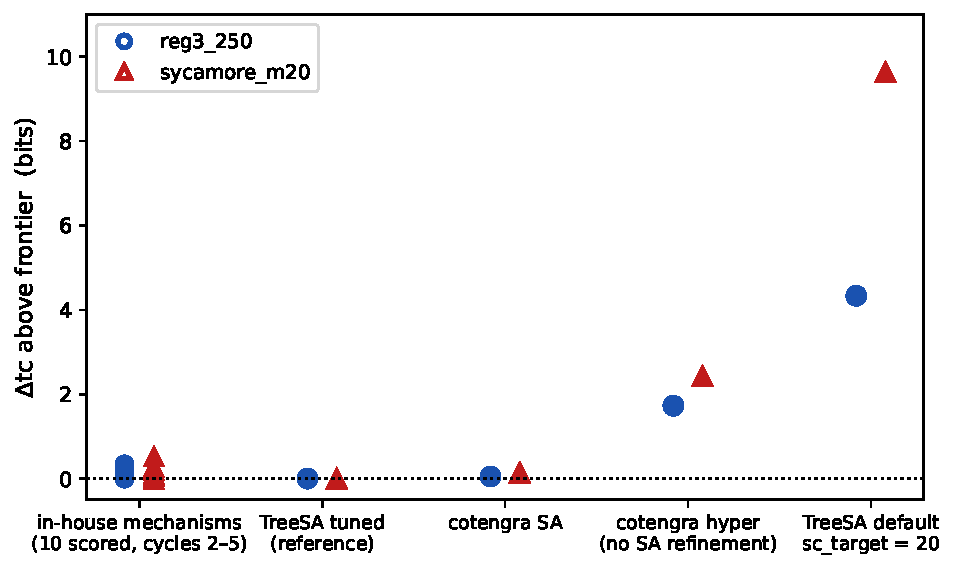
\includegraphics[width=\linewidth]{figures/fig2_frontier_convergence.pdf}
\caption{Distance $\Delta\tc$ from the frontier for every scored optimizer,
at matched 90-s single-thread budgets with validator-recomputed costs.
Open markers: ten in-house mechanisms (circles: \texttt{reg3\_250};
triangles: \texttt{sycamore\_m20}). Filled markers: reference rows. All
SA-refined optimizers---from either codebase---land within $0.5$ bits of the
frontier; hyper-optimization without SA refinement lags by $1.7$--$2.4$ bits;
the mis-tuned default baseline (Sec.~\ref{sec:masquerade}) lags by
$4$--$10$ bits.}
\label{fig:convergence}
\end{figure}

\begin{figure}[t]
\centering
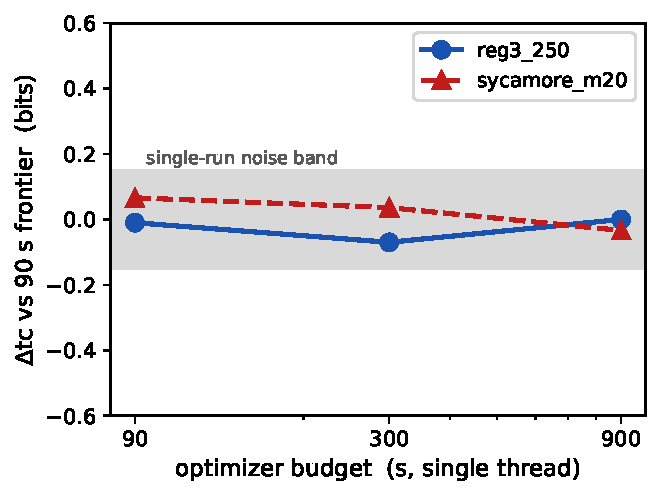
\includegraphics[width=0.72\linewidth]{figures/fig6_budget_scaling.pdf}
\caption{Budget independence of the frontier. Change in frontier $\tc$
relative to the 90-s value for tenfold longer optimizer budgets
(single runs; shaded band indicates single-run scatter).}
\label{fig:budget}
\end{figure}

\subsection{The mis-tuned-baseline trap}
\label{sec:masquerade}

The frontier was not established in one step, and the detour is itself a
result with practical consequences. In an early batch, eight novel
mechanisms each beat the then-current TreeSA reference by $4.3$ bits on
\texttt{reg3\_250} and by up to $9.7$ bits ($\approx 800\times$ in flops) on
\texttt{sycamore\_m20}---apparently a decisive algorithmic advance
(Fig.~\ref{fig:masquerade}). Two observations undermined that reading: the
eight mechanically unrelated searches clustered within $0.35$ bits of one
another, and an ablation attributed essentially the whole gain to a shared
objective change rather than to any specific move set. The explanation is a
default parameter: TreeSA's annealing objective in
\textsf{omeco}~\cite{omeco} (following the Julia implementation
\textsf{OMEinsumContractionOrders.jl}~\cite{oecorders}) targeted a
\emph{low} space complexity, $\texttt{sc\_target}=20$, appropriate for
memory-starved settings but active on instances whose feasible optimum sits at
$\sczz = 34$ and $53$: the sc pressure drags the search into
low-memory/high-flop regions. Re-measuring the \emph{stock} TreeSA with the
one-line change $\texttt{sc\_target}=\infty$ (pure-$\tc$; equivalently, the
memory cap when one exists) reproduced the entire improvement:
$44.29 \to 39.90$ and $71.17 \to 61.53$, retaking or tying every ``record''
the novel mechanisms had set. None of the eight mechanisms improves on the
correctly tuned baseline. The lesson generalizes the mis-tuned-baseline
critique of empirical machine learning to combinatorial optimizers:
\emph{apparent} algorithmic gains of nearly three orders of magnitude can be
manufactured by a single sub-optimal default in the reference. The practical
consequence---aspirational low-memory targets are harmful, and the harm is
one-directional---is now encoded in \textsf{omeco}'s defaults
(Sec.~\ref{sec:practice}).

\begin{figure}[t]
\centering
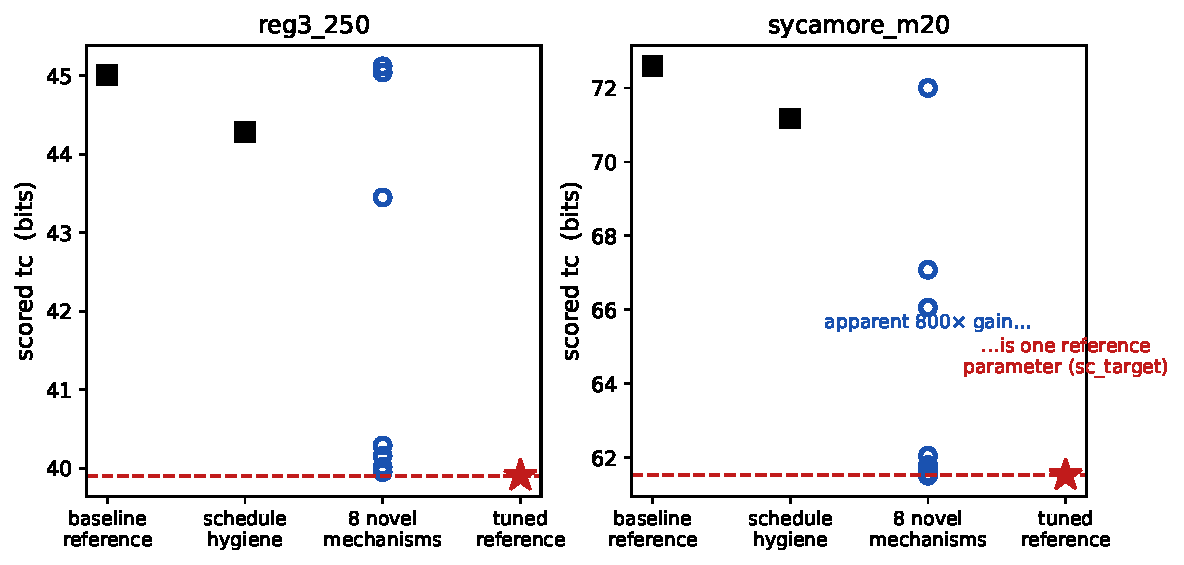
\includegraphics[width=\linewidth]{figures/fig3_sc_target_masquerade.pdf}
\caption{The mis-tuned-baseline trap. Scored $\tc$ of the original baseline
(squares), eight novel mechanisms (open circles), and the re-tuned stock
baseline (star, dashed line). The apparent up-to-$800\times$ algorithmic
improvement on \texttt{sycamore\_m20} is explained entirely by one baseline
parameter.}
\label{fig:masquerade}
\end{figure}

\section{Bracketing the optimum}
\label{sec:bounds}

We now bound the distance from the frontier to the true optimum
$\tc_{\mathrm{opt}} = \min_T \tc(T)$. All bounds are per-instance and carry
machine-checkable certificates; we distinguish \emph{certified} results
(rigorous, with verifiable artifacts) from \emph{structural} ones
(rigorous inequalities applied to a high-confidence extremal value found by
extensive search but not formally proven minimal).

\subsection{A sum-form isoperimetric bound}

Width-type bounds control the single largest contraction. But $\tc$ is a
log-sum over \emph{all} $n-1$ contractions, so we first derive a bound that
sees the sum. Let $b(k) = \min_{|S|=k} |\bnd{S}|$ denote the isoperimetric
profile of $G$.

\begin{theorem}[sum-form profile bound]
\label{thm:sumform}
For every binary contraction tree $T$ over the closed network $G$,
\begin{equation}
\tc(T) \;\ge\; \log_2 F(n),
\quad
F(n) = \min_{\text{tree shapes}} \sum_v 2^{b(|S_v|)},
\end{equation}
where the minimum ranges over all binary-tree size profiles and is computed
exactly by the dynamic program
$f(1)=0$, $f(k) = 2^{b(k)} + \min_{1\le j\le \lfloor k/2\rfloor}
[f(j)+f(k-j)]$, $F(n)=f(n)$. Replacing $b$ by any pointwise lower bound
$b_{\mathrm{lo}} \le b$ preserves validity.
\end{theorem}

The proof combines Lemma~\ref{lem:identity} termwise with the observation
that the internal-node sizes of any binary tree satisfy exactly the DP
recursion; the DP is validated against brute-force minimization over all tree
shapes for small $n$ and against closed forms for cycles. A certified
instantiation uses the spectral profile
$b_{\mathrm{spec}}(k) = \lambda_2\, k(n-k)/n \le b(k)$, with $\lambda_2$ the
algebraic connectivity, yielding certified bounds of $13.14$
(\texttt{reg3\_250}, $\lambda_2 = 0.2036$) and $9.84$
(\texttt{sycamore\_m20}, $\lambda_2 = 0.0462$) bits. A sharper,
high-confidence instantiation uses an empirical profile $b_{\mathrm{emp}}$
assembled from Fiedler sweeps, region growing, FM-style refinement, and cuts
harvested from real contraction trees, every cut independently re-verified;
it yields $30.81$ and $47.17$ bits (Fig.~\ref{fig:profiles}).

\begin{figure}[t]
\centering
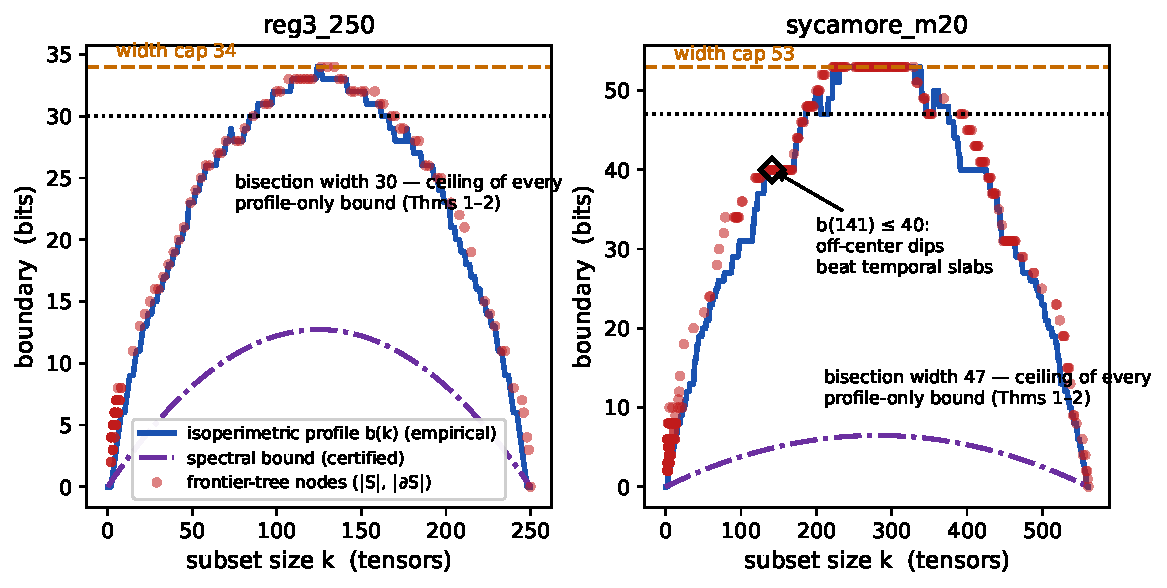
\includegraphics[width=\linewidth]{figures/fig4_profiles.pdf}
\caption{Isoperimetric profiles and what a real tree pays. Solid line:
empirical profile $b(k)$ (upper bound on the true profile; every cut
verified). Dash-dotted: certified spectral bound. Dots: the frontier tree's
own nodes $(|S_v|, |\bnd{S_v}|)$---a balanced tree is forced to pay a plateau
of near-maximal boundaries. Dotted line: bisection width, the provable ceiling
of every profile-only bound (Sec.~\ref{sec:impossibility}). Dashed line: the
achieved width. Diamond: the certified $b(141)\le 40$ cut, showing the
profile dips off-center below the 53-wire temporal slab.}
\label{fig:profiles}
\end{figure}

\subsection{Width certificates and the carving bracket}

For width-type bounds we use the exact correspondence between contraction
width and the treewidth of the line graph
$L(G)$~\cite{markov_2005_simulating}: every tree obeys
$\tc \ge \sczz \ge \mathrm{tw}(L(G))$ (in bits, up to the standard $+1$
convention). Minor-based lower-bound search~\cite{tamaki_2022_heuristic}
with certificates cross-checked by two independent exact
solvers~\cite{tamaki_2017_positive,strasser_2017_computing} certifies
\begin{equation}
\tc \ge 18 \;\; (\texttt{reg3\_250}),
\qquad
\tc \ge 22 \;\; (\texttt{sycamore\_m20}),
\end{equation}
far below the structural truth---certifying high treewidth on expander-like
line graphs is where current tooling saturates, a known frontier of the PACE
line of work.

The Sycamore proxy admits a much stronger structural argument. Any binary
tree on $n$ leaves has an edge whose leaf-set $S$ satisfies
$n/3 \le |S| \le 2n/3$; by Lemma~\ref{lem:identity} the contraction there
costs at least $|\bnd{S}|$, so
$\tc_{\mathrm{opt}} \ge B_{\mathrm{bal}}(G)$, the minimum balanced edge cut.
For the layered circuit graph the 53 qubit worldlines crossing any time slice
give an explicit balanced cut of exactly $53$; extensive search (multi-seed
METIS, Kernighan--Lin, and spatial/temporal sweeps) finds nothing smaller,
and the spatial cross-section ($\approx 70$) is well above it. Taking
$B_{\mathrm{bal}} = 53$ as a structural value:
\begin{equation}
\tc_{\mathrm{opt}}(\texttt{sycamore\_m20}) \;\in\; [53,\; 61.544],
\label{eq:bracket}
\end{equation}
and since real sc-53 trees exist, $\sczz = 53$ is \emph{width-optimal} and
$\mathrm{tw}(L(G)) = 52$ exactly. \textbf{Equation~\eqref{eq:bracket},
visualized in Fig.~\ref{fig:ladder}, is our second main result:} the frontier
sits within $8.5$ bits of the optimum on the Sycamore proxy, it is exactly
width-optimal, and the residual equals $\log_2$ of a counting factor,
$8.5 \approx \log_2 561 = 9.1$.

\begin{figure}[t]
\centering
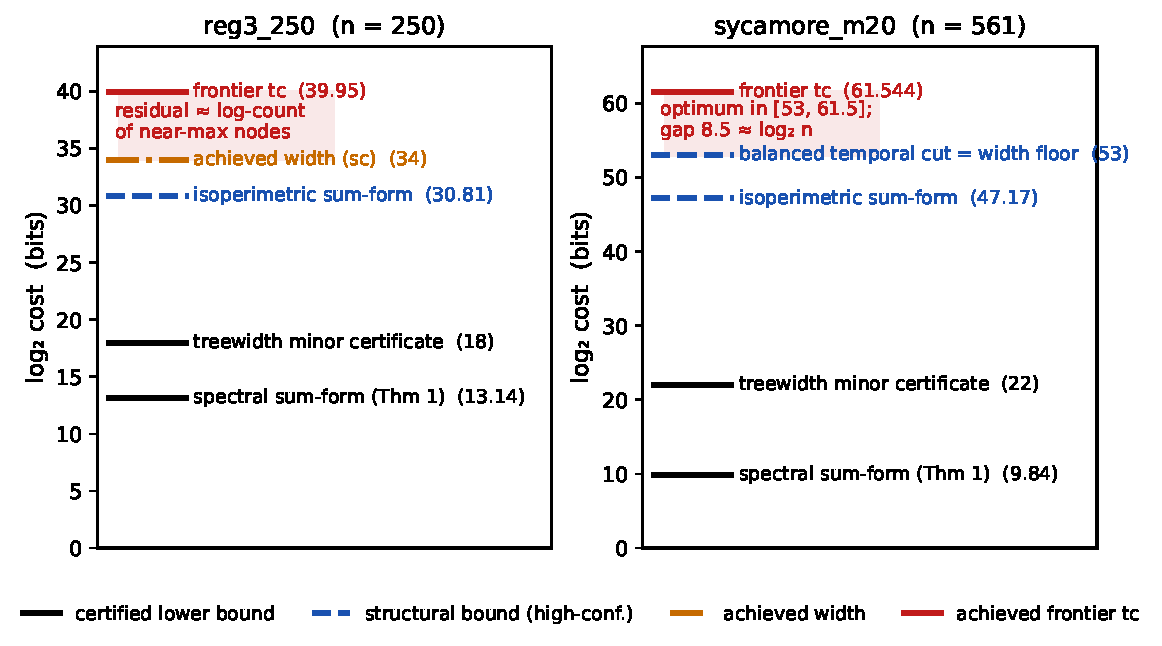
\includegraphics[width=\linewidth]{figures/fig1_certification_ladder.pdf}
\caption{The certification ladder. Every certified (solid) and structural
(dashed) lower bound, the achieved width (dash-dotted), and the achieved
frontier (red), on one $\log_2$-cost axis per instance. The shaded interval
on \texttt{sycamore\_m20} is the localized optimum,
Eq.~\eqref{eq:bracket}.}
\label{fig:ladder}
\end{figure}

\section{Why the residual resists width-type certification}
\label{sec:impossibility}

Is the remaining $8.5$-bit gap a weakness of our bounds or a structural
blind spot? We prove the latter, in two steps.

First, we strengthened Theorem~\ref{thm:sumform} to forbid the skewed tree
shapes that make its DP collapse:

\begin{theorem}[dyadic-window bound]
\label{thm:dyadic}
Follow the larger-child path from the root; for
$j = 1,\dots,\lfloor\log_2 n\rfloor - 1$ it visits at least one node whose
leaf-set size lies in the dyadic window $W_j = (n/2^{j+1},\, n/2^{j}]$, and
these nodes are distinct. Hence
$\tc(T) \ge \log_2 \sum_{j} 2^{\min_{k\in W_j} b(k)}$ for every $T$.
\end{theorem}

Both theorems are proven and validated (the DP against brute force; the
window argument on 3000 random trees), yet both \emph{collapse when
evaluated}: the unconstrained DP hides all cost in one balanced node
(its largest term is 57--89\% of the sum), and the dyadic sum is a
log-sum-exp over $\le \log_2 n$ terms, adding at most
$\log_2\log_2 n \approx 3$ bits over its largest---whose window minimum sits
at the \emph{off-center} end of the widest window. The certified cut
$b(141) \le 40$ on the Sycamore proxy (Fig.~\ref{fig:profiles}) pins this
down: compact spacetime boxes beat temporal slabs away from balance, so the
profile dips below the bisection width off-center.

\begin{observation}[profile bounds cap at the bisection width]
\label{obs:cap}
Both mechanisms above are instances of a general fact: any lower bound that
is a function of the isoperimetric profile $b(\cdot)$ alone is bounded by the
balanced-separator (bisection) value
$\max_{n/3\le k\le 2n/3}$-window minimum of $b$---here $47$
(\texttt{sycamore\_m20}) and $30$ (\texttt{reg3\_250})---which lies
\emph{below} the carving value $53$ and far below the frontier. The gap
between the bisection width and the optimum lives in the joint, nested
structure of the cuts a single tree must realize simultaneously, which the
per-size minima $b(k)$ cannot see.
\end{observation}

\textbf{Theorem~\ref{thm:dyadic} together with Observation~\ref{obs:cap} is
our third main result:} the profile-bound family is exhausted below the
frontier for structural, not computational, reasons; closing
Eq.~\eqref{eq:bracket} requires genuinely nested (carving-aware) sum-form
arguments, which we leave open.

The counting interpretation of the residual is corroborated from the
optimizer side. If the gap $\tc - \sczz \approx \log_2(\#\text{near-maximal
contractions})$ were slack, a search that targets the profile should flatten
it. Measured on trees of equal or better $\tc$
(Fig.~\ref{fig:conservation}), the opposite happens: reducing the peak node
cost by one bit \emph{fattens} the near-peak shelf ($7\to 19$ nodes on
\texttt{reg3\_250}, $5\to 17$ on \texttt{sycamore\_m20})---total flops behave
as conserved under profile reshaping. Profile-aware annealing accordingly
ties plain annealing exactly. At the frontier, the near-maximal multiplicity
is not slack; it is the price of width-optimality.

\begin{figure}[t]
\centering
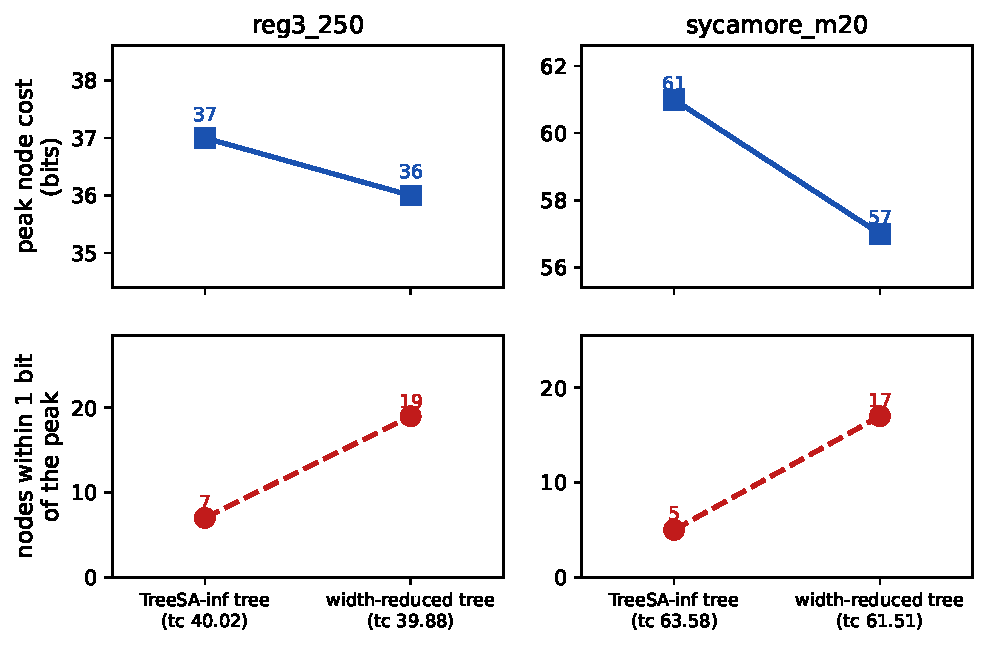
\includegraphics[width=0.9\linewidth]{figures/fig5_profile_conservation.pdf}
\caption{Profile conservation at the frontier. Between trees of equal or
better $\tc$, lowering the peak node cost (top row) fattens the near-peak
shelf (bottom row): the log-count residual is structural, not slack.}
\label{fig:conservation}
\end{figure}

\section{Practical consequences}
\label{sec:practice}

Three recommendations follow directly from the measurements.

\emph{(i) Never target a space complexity below the natural width of good
trees.} The harm of \texttt{sc\_target} is one-directional: on instances
whose min-$\tc$ trees have near-minimal $\sczz$ anyway (both instances here),
an unconstrained pure-$\tc$ objective loses nothing, while an aspirational
low-memory target costs up to $9.7$ bits. \textsf{omeco} now defaults to
unconstrained $\tc$ unless the user supplies a real memory budget, matching
the overflow-penalty-only design of~\cite{kalachev_2021_multi}.

\emph{(ii) At 90-second budgets, SA refinement is the differentiator, not
hyper-optimization.} Practitioners using \textsf{cotengra} on comparable
instances should enable its SA refinement; hyper-optimization alone
under-refines by $1.7$--$2.4$ bits here.

\emph{(iii) Single scored runs are meaningless at larger scales.} On
1000-tensor instances (measured in the same campaign), run-to-run variance
($\pm 1$--$5$ bits) exceeds real method differences; distribution reporting,
as practiced in~\cite{gray_2020_hyper}, is mandatory there.

\section{Methods}
\label{sec:methods}

The measurements were produced by an autonomous research loop with a strict
measurement protocol, run over six batches of independently implemented
attempts. Each attempt lives in its own git worktree with a hypothesis log
and a machine-readable score report; scoring is performed exclusively by a
sandboxed validator (network-denied, write-denied outside the worktree,
wall- and CPU-limited) that relabels the instance per run and recomputes all
costs from the emitted tree topology. Records require a confirmation run on
a fresh relabeling, recording the worse result. Negative controls---a
hardcoded-tree cheater, an over-threading burner, a timeout, an
environment-escape probe, and a wrong-answer emitter---are re-verified
against the validator after every harness change. The loop's reflection
step, not any single measurement, caught all three failure modes reported
here: the mis-tuned baseline (Sec.~\ref{sec:masquerade}), a scale-variance
illusion (local bests evaporating under scoring), and a harness bias (a
scorer recursion limit silently rejecting the deep trees that good
random-circuit orders need). Certificates for every bound---minor witnesses,
tree decompositions verified by two independent exact solvers, cut listings
with independent double-counts, and the DP validation suite---are shipped
with the audit trail (31 worktrees, 6 cycle reports) in the accompanying
repository.

\section{Conclusions}
\label{sec:conclusions}

We have measured, for two representative tensor networks, where the practical
frontier of contraction-order optimization lies, and certified how close to
optimal it is: twelve optimizers from two toolchains converge to one frontier;
on a Sycamore-scale circuit proxy that frontier is exactly width-optimal and
within $8.5 \approx \log_2 n$ bits of the true optimum; and the residual is
provably invisible to every bound built from the isoperimetric profile alone,
while behaving as a conserved quantity under search. The practical outputs
are a corrected default in a shipping library and a protocol---relabeling,
recomputed costs, confirmation runs, negative controls---that turned three
would-be discoveries into diagnosed artifacts.

Two open problems follow. Theoretically, closing Eq.~\eqref{eq:bracket}
requires sum-form bounds over \emph{nested} cut families (carving-aware
analogues of Theorem~\ref{thm:sumform}); the $47 \to 53 \to 61.5$ hierarchy
measured here says exactly how much each structural level is worth.
Empirically, extending certification to larger instances requires
variance-aware protocols before optimizer differences can even be resolved.
We suggest that benchmark suites for contraction-order optimizers adopt
per-instance certified brackets---not only optimizer-vs-optimizer
deltas---as the standard of evidence.

\begin{acknowledgments}
The measurement campaign, including all attempt implementations, bounds,
certificates, and reports, was executed by an autonomous AI research loop
(Claude, Anthropic) under the author's direction, with every scored result
produced by the sandboxed validator described in Sec.~\ref{sec:methods}.
[Funding acknowledgments to be added.]
\end{acknowledgments}

\bibliographystyle{unsrt}
\bibliography{references}

\end{document}
